\documentclass{report}

\usepackage{graphicx}
\usepackage{etoolbox}
\usepackage{titlesec}
\usepackage{amssymb}

\titleformat{\chapter}[display]
  {\normalfont\bfseries}{}{0pt}{\Huge}
\titlespacing*{\chapter}{0pt}{-50pt}{40pt}
	
\newcommand*{\titleGM}{\begingroup 
\hbox{
\hspace*{0.2\textwidth} 
\rule{1pt}{\textheight} 
\hspace*{0.05\textwidth} 
\parbox[b]{0.75\textwidth}{ 

{\noindent\Huge\bfseries User Manual}\\[2\baselineskip]
{\large \textit{Absolute Concentration Robustness Exploration (ACRE)}}\\[4\baselineskip] 
{\Large \textsc{Xin Gao, Islam Almasri, Ramzan Umarov}}

\vspace{0.5\textheight} 
{\noindent November, 2016}\\[\baselineskip] 
}}
\endgroup}


\graphicspath{{./figs/}}

\patchcmd{\thebibliography}{\chapter*}{\section*}{}{}
\AtBeginDocument{\renewcommand{\bibname}{Reference}}

 


\begin{document}
\titleGM 
\thispagestyle{empty}
\newpage
\tableofcontents
\thispagestyle{empty}
\newpage
\vspace{-2cm}
\chapter{HOW TO INSTALL}
\section{Requirements}
The program is packaged as an executable JAVA file, to run it, you need JAVA Runtime Environment downloaded. To download JAVA, please go to the following website:  www.java.com/getjava/

Any Operating System is sufficient to run the software as long as it has a JAVA Runtime Environment available for it. Once you have JAVA 1.6 or above installed you should be able to run the application by typing the following command in Command of Windows or Terminal of Mac OS or Linux:

java -jar ACRE.jar

\section{Package Contents}
The Package contains the following:
\begin{enumerate}
	\item Modules: a folder containing sample SBML files for frequently-seen modules. 
  \item Workspaces: a folder containing sample workspaces. 
  \item ACRE.jar: the executable application file. 
  \item UserManual\textunderscore ACRE.pdf: this user manual. 
\end{enumerate}
\vspace{-2cm}
\chapter{SYSTEM SUMMARY}
\section{Functionality}

The overall idea of ACRE is to enumerate all the biochemical reaction networks that consist of
user-created nodes from user-selected modules under user-specified constraints; to apply
Shinar and Feinberg's theorem \cite{c1}; and to determine which of the networks have the absolute
concentration robustness (ACR) property.

\section{Workflow}
ACRE is a JAVA-based system that has been tested on Windows 7, Mac OS X 10.8, and Ubuntu
11.10. ACRE requires JAVA 1.6 or above. The workflow of the software is illustrated in Fig~\ref{fig:1}.


\underline{Step 1}: ACRE reads modules in the System Biology Markup Language (SBML) format. ACRE
extracts \textit{reactions}, \textit{reactants}, \textit{products} and \textit{stoichiometry} from SBML files for the analysis of the
ACR property. ACRE provides a number of basic, frequently-seen modules. Alternatively, the
user can create/import their own modules as long as their SBML files contain the required
information.


\underline{Step 2}: Once a module is loaded, the user specifies the input and output species of the module.
An input species is a reactant or a product that can be replaced by an external output species,
and an output species is a reactant or product that can replace an external input species. The
input and output species cannot be the same for the same module. This restriction is to prevent
invalid networks to be constructed. In the case that the user wishes to specify different inputs
and outputs for a particular module, that module can be loaded multiple times. The user then
creates as many realizations of modules as needed, each of which is referred to as a node in our
tool.


\underline{Step 3}: Two types of constraints can be used to restrict the composition of networks, i.e., \textit{local
constraints} and \textit{global constraints}. Local constraints are set to each node, and these constrain
the way in which nodes are connected to build networks. By default, the local constraints are set
to ``no connection'', which means that the outputs of a node cannot be connected to any other
node. Global constraints are defined at the network level. The user can specify the minimum
and maximum number of connection edges that the network can possess. Global constraints
can prevent the construction of over-sparse or over-dense networks, and also limit the search
space of all possible networks in order to achieve improved computational efficiency.


\underline{Step 4}: For analysis of the results, the user can select the information to be generated in the
report. This can include runtime, the number of constructed networks, and the number of
networks with ACR. The tool can provide an output of the networks with ACR in SBML, and
specify which of the species in each of these networks have the ACR property. The report can be
displayed on screen and saved to a file. Furthermore, the workspace can be saved or loaded at
any time for future use. ACRE also supports restricted search. The user can specify which species
is desired to have ACR. The tool will thus report only those networks that have ACR on the
specified species.


\underline{Step 5}: ACRE enumerates all the possible networks with the created nodes under user-specified
constraints. For each network, the tool applies Shinar and Feinberg's theorem to
deterministically identify which species have ACR. Once all the networks are enumerated, the
results are summarized and a report is generated.

\begin{figure}
	\centering
		
\includegraphics[width=0.8\textwidth]{1}
	\caption{Workflow of ACRE}
	\label{fig:1}
\end{figure}
\vspace{-2cm}
\chapter{USER INTERFACE GUIDE}
\section{Example}
In this section, an overview of the user interface will be provided, with a step-by-step example
illustration. The following example is a chemical reaction network presented in \cite{c1}, which is
known to have ACR on species \textit{C}, Fig~\ref{fig:2}.

\begin{figure}
	\centering
		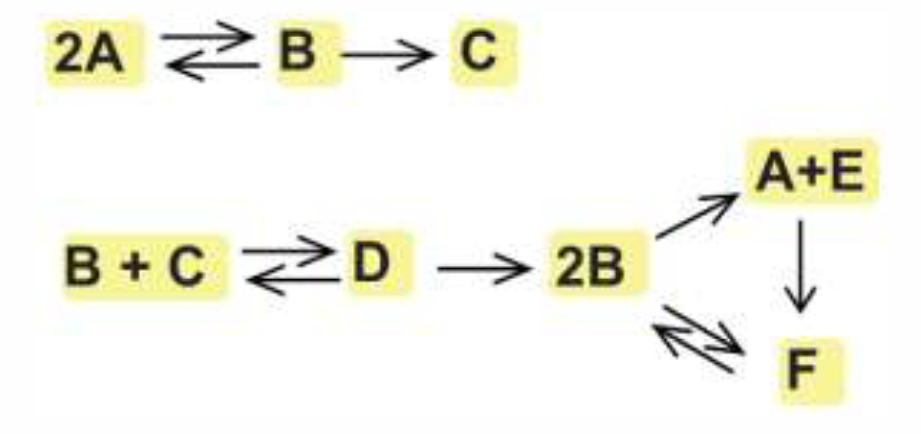
\includegraphics[width=0.3\textwidth]{2}
	\caption{Example chemical reaction network with ACR on \textit{C} (figure taken from \cite{c1})}
	\label{fig:2}
\end{figure}

Suppose one has created four SBML files for this network. Those are:

$M1: 2A \leftrightarrows  B \rightarrow C$

$M2: B + C \leftrightarrows  D \rightarrow 2B$

$M3: A + E \rightarrow F$

$M4: 2B \rightarrow A + E, 2B \leftrightarrows  F$

Note that the same letter in different modules does not necessarily denote the same species.
We now demonstrate how to apply ACRE to further investigate the structural features of ACR
with respect to these modules. Once ACRE is opened, the main window is shown as in Fig~\ref{fig:3}.

\begin{figure}
	\centering
		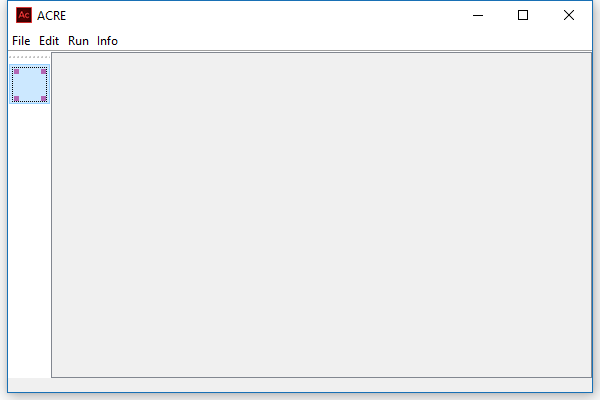
\includegraphics[width=0.6\textwidth]{3}
	\caption{The main window of ACRE. The top panel is the menu bar, the left panel is the
module bar, and the right grey panel is the node space for created nodes.}
	\label{fig:3}
\end{figure}

\section{Load Modules}

The first step is to import SBML files that represent the modules of the desired chemical
reaction network. To find out more about SBML representation and how to create SBML files,
please refer to the website: http://sbml.org/.


In this example, we load the pre-prepared SBML files provided within the package. To open
these files:

\begin{enumerate}
	\item Click File $\rightarrow$ Load
	\item Navigate to SBML/EX2a.xml
	\item Open
	\item Open EX2b.xml, EX2c.xml, and EX2d.xml in the similar way
\end{enumerate}

\section{Module IO Selection}
After opening the SBML file the Module IO Selection window will appear. See Fig~\ref{fig:4}.

\begin{figure}
	\centering
		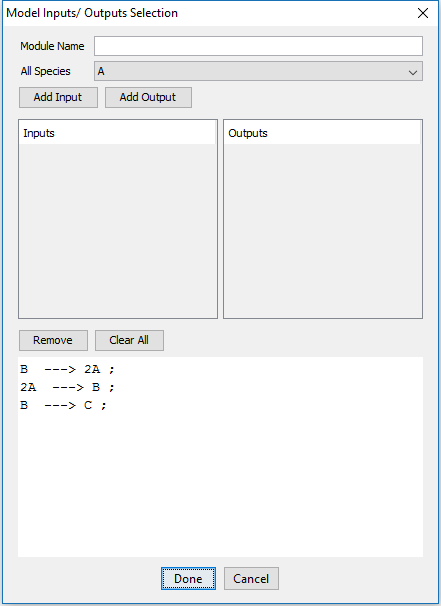
\includegraphics[width=0.5\textwidth]{4}
	\caption{Module IO selection window.}
	\label{fig:4}
\end{figure}

Note that in the white area at the bottom of this window, the reactions are listed, which
correspond to \textit{module1 (M1)}.

In this window, we define which of the species in the reactions should be inputs and outputs. To
do that, choose the species from the drop down menu, then click the corresponding button
(either Add Input, or Add Output).

In this example, we set the following inputs and outputs for the four modules:

\begin{table}[]
\centering
\label{tab:1}
\begin{tabular}{|l|l|l|}
\hline
   & Inputs & Outputs \\ \hline
M1 & A, B   & C       \\ \hline
M2 & C      & B       \\ \hline
M3 & A, E   & F       \\ \hline
M4 & B, F   & A, E    \\ \hline
\end{tabular}
\end{table}

Then click on ``Done''. We will see that four modules appear in the module bar as shown in
Fig~\ref{fig:5}.

\begin{figure}
	\centering
		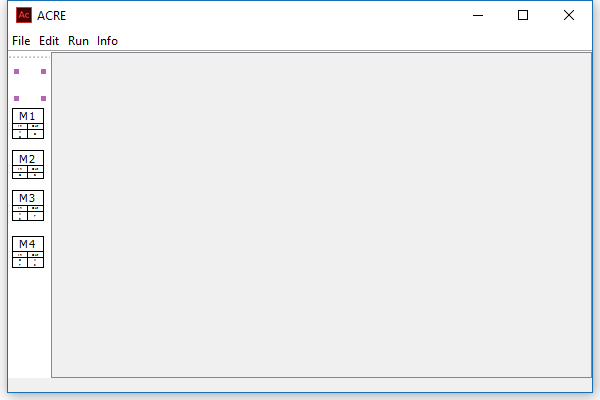
\includegraphics[width=0.6\textwidth]{5}
	\caption{ACRE window with the four modules loaded.}
	\label{fig:5}
\end{figure}

Note that ACRE will auto-generate a name for the module if none was given. Once a module is
created, one can delete the module, by selecting the icon representing the module in the
module bar, then choose Edit $\rightarrow$ Delete Module.

\section{Create/Delete/Move Nodes}

After creating modules, we need to create nodes. A node is a realization of a module. One can
create as many nodes as needed for any module.

To create a node, click on the module icon from the tool bar, then click anywhere in the node
space, a node will appear, with the following information shown:
\begin{enumerate}
	\item An auto-generated node name;
	\item The module from which the node is created;
	\item The lists of input and output species of this node.
\end{enumerate}

In this example, we create one node for each module, as shown in Fig~\ref{fig:6}.

\begin{figure}
	\centering
		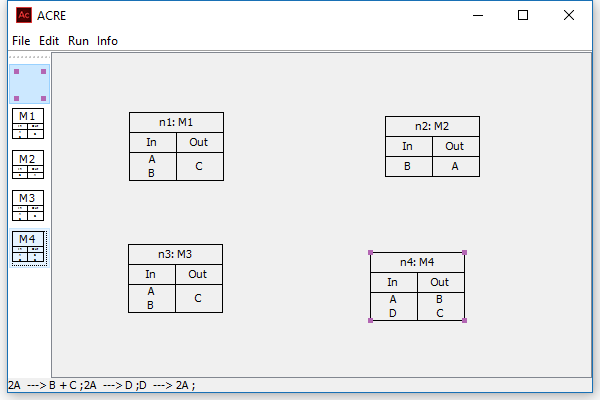
\includegraphics[width=0.6\textwidth]{6}
	\caption{ACRE window with four nodes created.}
	\label{fig:6}
\end{figure}

One can always move each node by first selecting the move tool from the module bar, which is
the first tool showing 4 squares in the corners. To move a node:
\begin{enumerate}
	\item Select the move tool from the module bar;
	\item Drag and drop the required node.
\end{enumerate}
To delete a node:

\begin{enumerate}
	\item Select the move tool from the module bar;
	\item Click on the required node, you will notice 4 small squares appearing on the corners;
	\item Choose Edit $\rightarrow$ Delete Node.
\end{enumerate}

\section{Set Constraints}

Each Node is associated with a set of local constraints regarding its inputs. To view/edit these
constraints, select the node and then choose Edit $\rightarrow$ Constraints, the ``Node Constraints
Selection'' window will appear as shown in Fig~\ref{fig:7}.

\begin{figure}
	\centering
		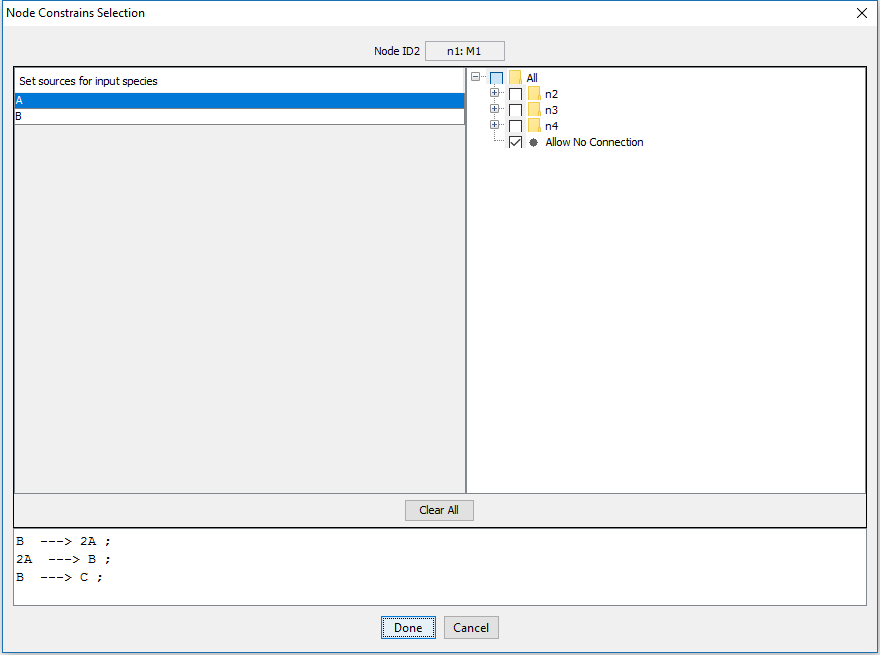
\includegraphics[width=0.95\textwidth]{7}
	\caption{Local constraint selection window.}
	\label{fig:7}
\end{figure}

From this window one can choose for each input of the node which outputs of other nodes can
be connected to it, and whether it can be left unconnected. A list of reactions will also appear in
the text box at the bottom. Note that the user has to set the constraints for all the inputs
species of all the nodes. Otherwise, the constraint will be set to no connection by default.

In this example, we require each input of each node must be connected by at least one output
from other nodes. Thus, ``Allow No Connection'' option is disabled.

Global constraints are optional to prevent the tool from generating over-sparse or over-dense
networks (Fig~\ref{fig:8}). By default, the minimum number of edges is 0 and the maximum is
2,147,483,647.

\begin{figure}
	\centering
		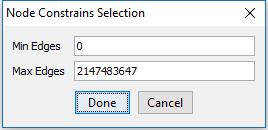
\includegraphics[width=0.5\textwidth]{8}
	\caption{Global constraint selection window.}
	\label{fig:8}
\end{figure}

\section{Save/Load Workspace}
At any point one can save the workspace which constitutes of:
\begin{enumerate}
	\item The modules created;
	\item The nodes created;
	\item The constraints.
\end{enumerate}

Saving/Loading the workspace comes in handy in case the user needs to modify the network
later. To save/load network, use the corresponding menu item from the file menu.

\section{Set Report Options}
The final step is to enumerate and analyze all the networks that satisfy the specified local and
global constraints. To do that, choose Run $\rightarrow$ Enumerate. Before the enumeration starts, the
``Enumeration Options'' window will appear as in Fig~\ref{fig:9}.

\begin{figure}
	\centering
		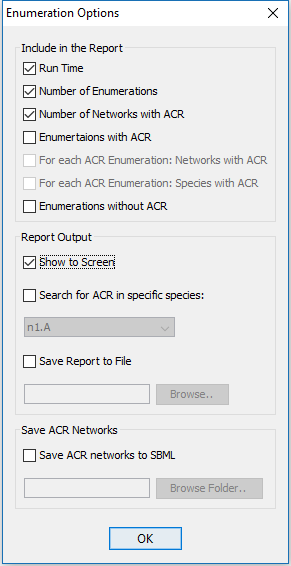
\includegraphics[width=0.4\textwidth]{9}
	\caption{Enumeration options window.}
	\label{fig:9}
\end{figure}

This window enables the user to select what should be included in the output. Make sure not to
include the details of the enumeration in this step in the cases where a huge number of
networks are anticipated.

In this example, we select to display the runtime, the total number of networks enumerated and
analyzed, the number of networks that have ACR. We select to show such information on
screen.

\section{Enumerate and Analyze}

Once the report options are set, we click OK button, which will start the enumeration and
analysis process. After the whole process is finished, the desired report is displayed on screen as
shown in Fig~\ref{fig:10}.

\begin{figure}
	\centering
		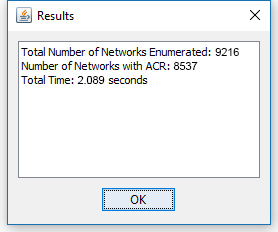
\includegraphics[width=0.4\textwidth]{10}
	\caption{Output report.}
	\label{fig:10}
\end{figure}

Interestingly, by allowing different ways to connect these four nodes, there are 9,216 networks
in total, 8,537 of which have ACR species. ACRE is able to finish the enumeration and analysis
process for this large number of networks in just 2 seconds.

\section{Restricted Search}
The user can specify which species is desired to have ACR. The tool will thus report only those
networks that have ACR on the specified species.

In this example, if we restrict species A of \textit{node1} to have ACR, only 289 networks are found to
satisfy such requirement, as shown in Fig~\ref{fig:11}.

\begin{figure}
	\centering
		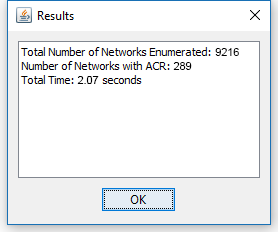
\includegraphics[width=0.4\textwidth]{11}
	\caption{Output report for restricted search.}
	\label{fig:11}
\end{figure}

\section{Scalability}

Fig~\ref{fig:12} shows the scalability of ACRE in terms of runtime and number of networks, from
which an approximately linear relationship can be observed.

\begin{figure}
	\centering
		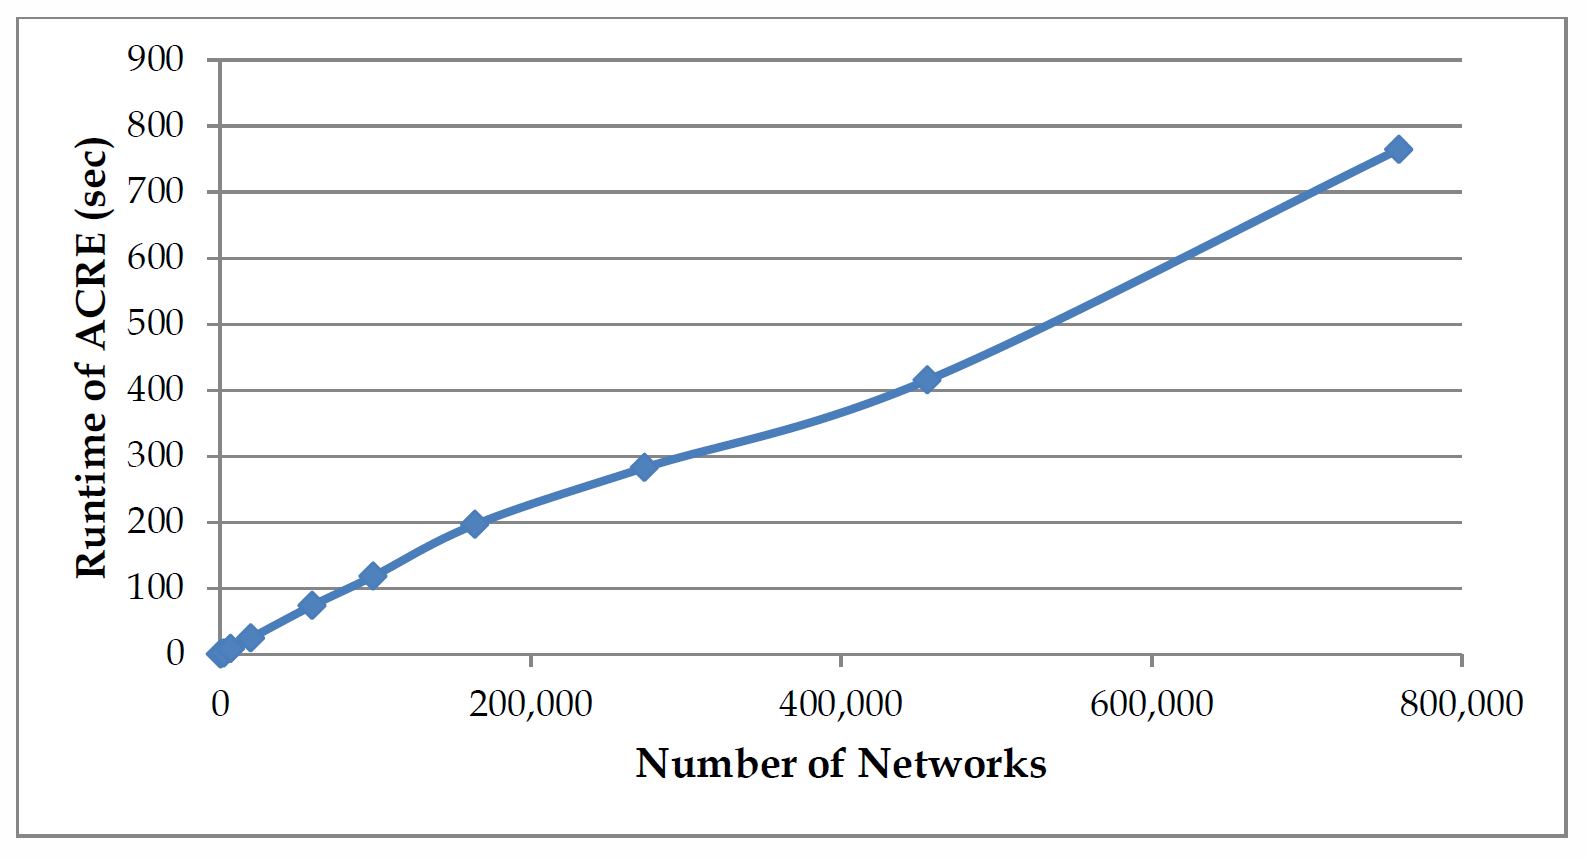
\includegraphics[width=0.8\textwidth]{12}
	\caption{Runtime v.s. number of networks.}
	\label{fig:12}
\end{figure}

\bibliographystyle{plain}
\bibliography{main}

\end{document}